%
% File acl2015.tex
%
% Contact: car@ir.hit.edu.cn, gdzhou@suda.edu.cn
%%

%% Based on the style files for EACL 2006 by 
%%e.agirre@ehu.es or Sergi.Balari@uab.es
%% and that of ACL 08 by Joakim Nivre and Noah Smith

\documentclass[11pt]{article}
\usepackage{times}
\usepackage{url}
\usepackage{latexsym}
\usepackage{listings}
\usepackage{graphicx}
\graphicspath{ {images/}}
\lstset{
   breaklines=true,
   basicstyle=\ttfamily}
%\setlength\titlebox{5cm}

% You can expand the titlebox if you need extra space
% to show all the authors. Please do not make the titlebox
% smaller than 5cm (the original size); we will check this
% in the camera-ready version and ask you to change it back.


\title{Rich Text Competition}

\author{Giwon Hong \\
  IR \& NLP Lab \\
  KAIST \\
  Daejeon, South Korea \\
  { gch02518@kaist.ac.kr} \\\And
  Minh-Son Cao \\
  IR \& NLP Lab \\
  KAIST \\
  Daejeon, South Korea \\
  { minhson@kaist.ac.kr} \\\And
  Haritz Puerto-San-Roman \\
  IR \& NLP Lab \\
  KAIST \\
  Daejeon, South Korea \\
  { haritzpuerto94@kaist.ac.kr} \\}

\date{}

\begin{document}
\maketitle

\section{Introduction}
Datasets are very valuable resources when doing research. However, it is not easy to find who else worked with that data, on what topics and with what results. Therefore, there is a waste of time and resources looking for related works using a specific dataset and what is more, some useful publications are underused. This work is the first step to tackle this problem. We proposed a model to retrieve dataset mentions, research fields and research methods from scientific publications. Our main approach to solve them is reading comprehension, named entity recognition, and TF-IDF similarity.

\section{Related works}
%\textbf{Question Answering} The state of the art in Question Answering is being continuously improved. The language model BERT \cite{devlin2018bert} was applied to QA and achieved a performance really close to humans in SQuAD dataset. Because of this, part of the research community want to shift the focus to speed rather than performance \cite{seo2018phrase}.

\textbf{Datasets retrieval} Although \textit{Information Retrieval} is a well established research field, only few attempts have focused on the task of dataset extraction form publications.  \cite{ghavimi2016identifying} tried it using heuristics and dictionaries but their heuristics have some problems. Firstly, they give too much weight to acronyms. For example, \textit{NYPD, (New York Police Department)} is detected as a dataset name. Furthermore, they also give an too much weight to the publication year of the datasets because they assumed dataset names are usually followed by the publication year but that may only work on Social Sciences publications. For example, in the Computer Science datasets do not appear followed by the publication year so this heuristic cannot detect all kind of dataset mentions.

\section{Models}
In this section, we will explain about the models we use for datasets retrieval, research fields retrieval, and research methods retrieval.
\subsection{Datasets Retrieval}
Our approach to solve the dataset retrieval task is reading comprehension (RC) with query generation and entity typing. An RC model is applied to the given publications with our own query generation module. Then, the result from the RC model is filtered with an entity typing module. Figure \ref{fig: docqaarch } shows our overall approach for dataset retrieval. In following subsections RC model, query generation, and entity typing are explained in detail.


\begin{figure*}[!htb]
    \centering
    \includegraphics[width = 16cm]{{docqaarch3}}
    \caption{Overall architecture for dataset retrieval.}
    \label{fig: docqaarch }
\end{figure*}


\subsubsection{Document QA}
Reading comprehension models are neural networks that find answers for given queries according to a text. Answers must appear explicitly in the text. Since the dataset retrieval task is about finding explicit dataset mentions from publications, RC models are suitable for this task.

The RC model used in this work is Document QA \cite{clark2017simple}. It uses Bi-GRU, bi-attention, and self-attention mechanism. In addition, Document QA performs a paragraph selection that pre-filters and selects the \textit{k} most relevant paragraphs through TF-IDF similarity between the query and paragraphs. We observed that datasets are usually mentioned together in some specific paragraphs of the publications. Therefore, this model is appropriate for this task thanks to its paragraph selection stage.


\subsubsection{Query generation module} \label{sec:questiongen}
In order to apply an RC model (such as Document QA) to the dataset retrieval task, queries that are suitable for finding the datasets are required. However, defining a general query for retrieving datasets is difficult, since the dataset mentions appear in various form like surveys, datasets, or studies. Therefore, we devised a query generation module with some important query terms to generate multiple specific queries instead of one general query.

To generate important query terms, we used a query generation model that creates queries given answers proposed by \cite{yuan2017machine}. Thanks to this model, we could obtain a list of queries to retrieve datasets from the training set. After that, we extracted query terms that are frequent in the list of queries and at the same time are not frequent in non-dataset-mention sentences. Because of this, these query terms have discrimination power for retrieving dataset mentions since 1) queries are generated to extract mentions and 2) the query terms do not appear in the sentences without dataset mentions.

This list of query terms is used to generate a general query concatenating query terms. This query is used for the paragraph selection stage of Document QA, as shown in figure 1. After this stage, the query generation module generates queries for each paragraph by string matching, in order to create specific queries for each paragraph.

\subsubsection{Ultra-Fine Entity Typing}
Ultra-Fine Entity Typing \cite{Choi:2018:ACL} can predict a set of free-from phrases like \textit{criminal} or \textit{skyscraper} given a sentence with an entity mention. For example, in the sentence: \textit{Bob robbed John and he was arrested shortly afterwards}, Bob is of type \textit{criminal}. In our task, candidate answers proposed by Document QA and their context are input to Ultra-Fine Entity Typing.
Although this system can predict 10k different entity types in which \textit{dataset} is included, after a few experiments we observed that most of the dataset names are recognized as some specific entity types such as \textit{organization} and \textit{agency}. Since these entity types are consistent, we decided that this could be a feature for our candidate answer classifier.

\subsubsection{Candidate Answer Classifier}
Using the score given by RC model for each candidate answer and the entity types given by Ultra-Fine Entity Typing for each candidate answer, a neural network classifier that filters the candidate answers of Document QA was used. We discovered that a candidate answer with a high score given by Document QA and whose entity type is \textit{organization} or something similar is considerably likely to be a correct dataset name. Due to this pattern we were able to create neural network classifier to filter out candidate answers.

The classifier has the following architecture:
\begin{enumerate}
    \item Input size: 10332 (10331 labels from Ultra-Fine Entity Typing and the Document QA score)
    \item 1 hidden layer with 50 neurons
    \item Output size: 2
\end{enumerate}

The training set consists of 25172 examples and test set of 6293 examples. Adam optimizer was used and cross entropy was used as loss function.

\subsection{Research Fields Retrieval}

Our approach to get the research fields is based on TF-IDF similarity with Wikipedia articles. First, a set of Wikipedia articles about different research fields using the library MediaWiki\footnotemark for Python was obtained. The list of research fields provided the Coleridge Initiative for the Rich Context Competition was used to crawl Wikipedia. This list has three levels of hierarchy as the example in the  figure \ref{fig:researchfieldshiearchy}.

\footnotetext{https://www.mediawiki.org/wiki/MediaWiki}

\begin{figure}[!htb]
    \centering
    \includegraphics[width = 7cm]{{fieldshierarchy2.png}}
    \caption{Research fields hierarchy}
    \label{fig:researchfieldshiearchy}
\end{figure}

The leaf nodes of that hierarchy were searched in Wikipedia to retrieve specific research fields instead of general ones. For example: we were aiming to retrieve \textit{Neurosurgery} instead of \textit{Medicine}. 

Then, using Scikit-learn \cite{scikit-learn}, a TF-IDF matrix of all the publications and Wikipedia articles of research fields was computed and the research field and all its superior nodes in the hierarchy associated to the most similar article were returned along with the similarity in the range [0,1]. The overall architecture can be seen in figure \ref{fig:researchfields}.

\begin{figure}[!htb]
    %\centering
    \includegraphics[width = 7.5cm]{{researchfields2.png}}
    \caption{Overall architecture for research fields retrieval}
    \label{fig:researchfields}
\end{figure}

\subsection{Research Methods Retrieval}
For the research methods retrieval task, we modeled it as an named-entity recognition (NER) problem. Research methods are considered to be an named entity and because of this, they can be tagged as research method label (RS) instead of common NER labels such as: \textit{location}, \textit{people}, etc. Figure \ref{fig:research_method} shows the main architecture of the model proposed by \cite{lample2016neural} and used in this task.

\begin{figure}
    \centering
    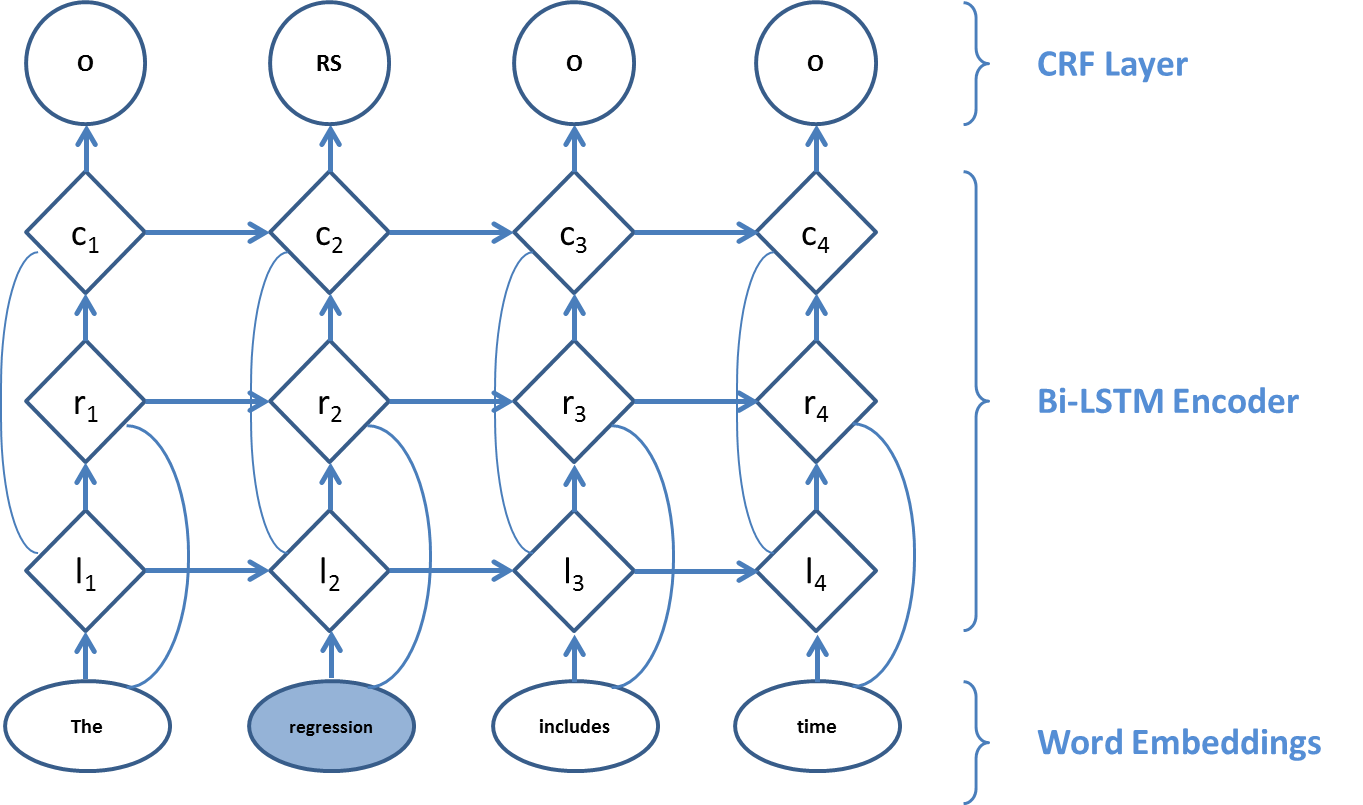
\includegraphics[width = 7.5cm]{bi-lstm.png}
    \caption{BiLSTM-CRF architecture}
    \label{fig:research_method}
\end{figure}

The representation of a word using the model is obtained  considering its context. We have the assumption that research methods have dependencies and constraints with words that appear in their surrounding context. Therefore, the conditional random field \cite{lafferty2001conditional} layer in this model is suitable for detecting research methods by jointly tagging the whole sentence, instead of independently tagging each word.

In this task, research method phrases which appeared in the training set were marked. Then, we represented the data in CoNLL 2003 format \cite{tjong2003introduction}, using IOB tag (Inside, Outside, Beginning). Every token is labeled as B-RS if the token is the beginning of a research method, I-RS if it is inside a research method but not the first token, or O if otherwise. We used this type of data to train the model which could detect research methods in publications. 

\section{Experiment}
The Coleridge Initiative released a labeled training set of 5000 publications and a labeled dev set of 100 publications in the phase 1 of the Rich Context Competition. After the end of the phase 1, a labeled holdout set of 5000 publications of phase 1 and another unlabeled training set of 5000 publications of phase 2 was also released. For training, we use 5000 publications from phase 1 training set and another 5000 publications from phase 1 holdout set. 

The experiment was performed using Docker\cite{anderson2015docker} on an Amazon Web Services (AWS) T2 2xlarge instance which contains 8 virtual CPU cores and 32GB memory without GPU. 

\section{Results and Discussions}
Due to the difficulty of performing a quantitative analysis on a not extensively labeled dataset, a qualitative analysis was made. Several random publications were chosen and manually labeled by us to check the quality of our model and discover the strong and weak points.

\subsection{Datasets Retrieval}
To analyze the effects of the query generation module and entity typing module, we performed analyses on 100 phase 1 dev set with 3 different settings:
\begin{enumerate}
    \item Document QA only
    \item Document QA + query generation module
    \item Document QA + query generation module + entity typing module
\end{enumerate}

\subsubsection{Document QA only}
Figure \ref{fig:docqaonly} shows the results from 3 publications of phase 1 dev set with Document QA only. Compared to the other settings, Document QA only setting retrieves answers (dataset mentions) with high quality. However, the number of  retrieved answers is notably small. For example, the result from \textit{153.txt} publication was empty as in figure \ref{fig:docqaonly}. In fact, our model using this setting can retrieve only 260 answers (predictions) from 100 publications of phase 1 dev set.

\begin{figure}[!htb]
    \centering
    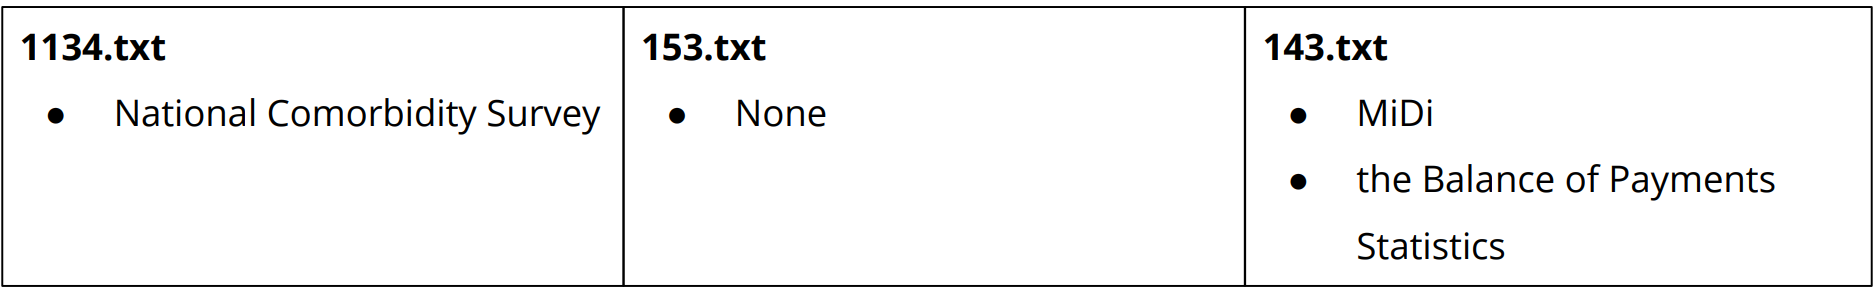
\includegraphics[width = 8cm]{phase1.png}
    \caption{Results from Document QA only}
    \label{fig:docqaonly}
\end{figure}

These results with fewer answers were expected, due to the difficulty of defining general queries as explained in section \ref{sec:questiongen}. Without a query generation module, our query was not representative enough to retrieve various forms and types of the dataset mentions.

\subsubsection{Document QA + query generation module}
Figure \ref{fig:docqaquery} shows the results from 3 publications of phase 1 dev set with Document QA and query generation module. Because of the latter, our dataset retrieval model could retrieve a large number of answers. For example, the result from \textit{153.txt} publication contains a large number of answers with correct answers such as \textit{financial services FDI data} or \textit{Micro Batabase Direct investment}. Therefore, we believe that the query generation module improves recall of the entire dataset retrieval model. Actually, our model using this setting can retrieve more than 2,000 answers (predictions) from 100 publications of phase 1 dev set.

However, compared to the Document QA only setting, there is a considerable number of noise. For example, in figure \ref{fig:docqaquery}, \textit{empirical, Table 1, Section 4} and etc., are not dataset mentions. 

\begin{figure}[!htb]
    \centering
    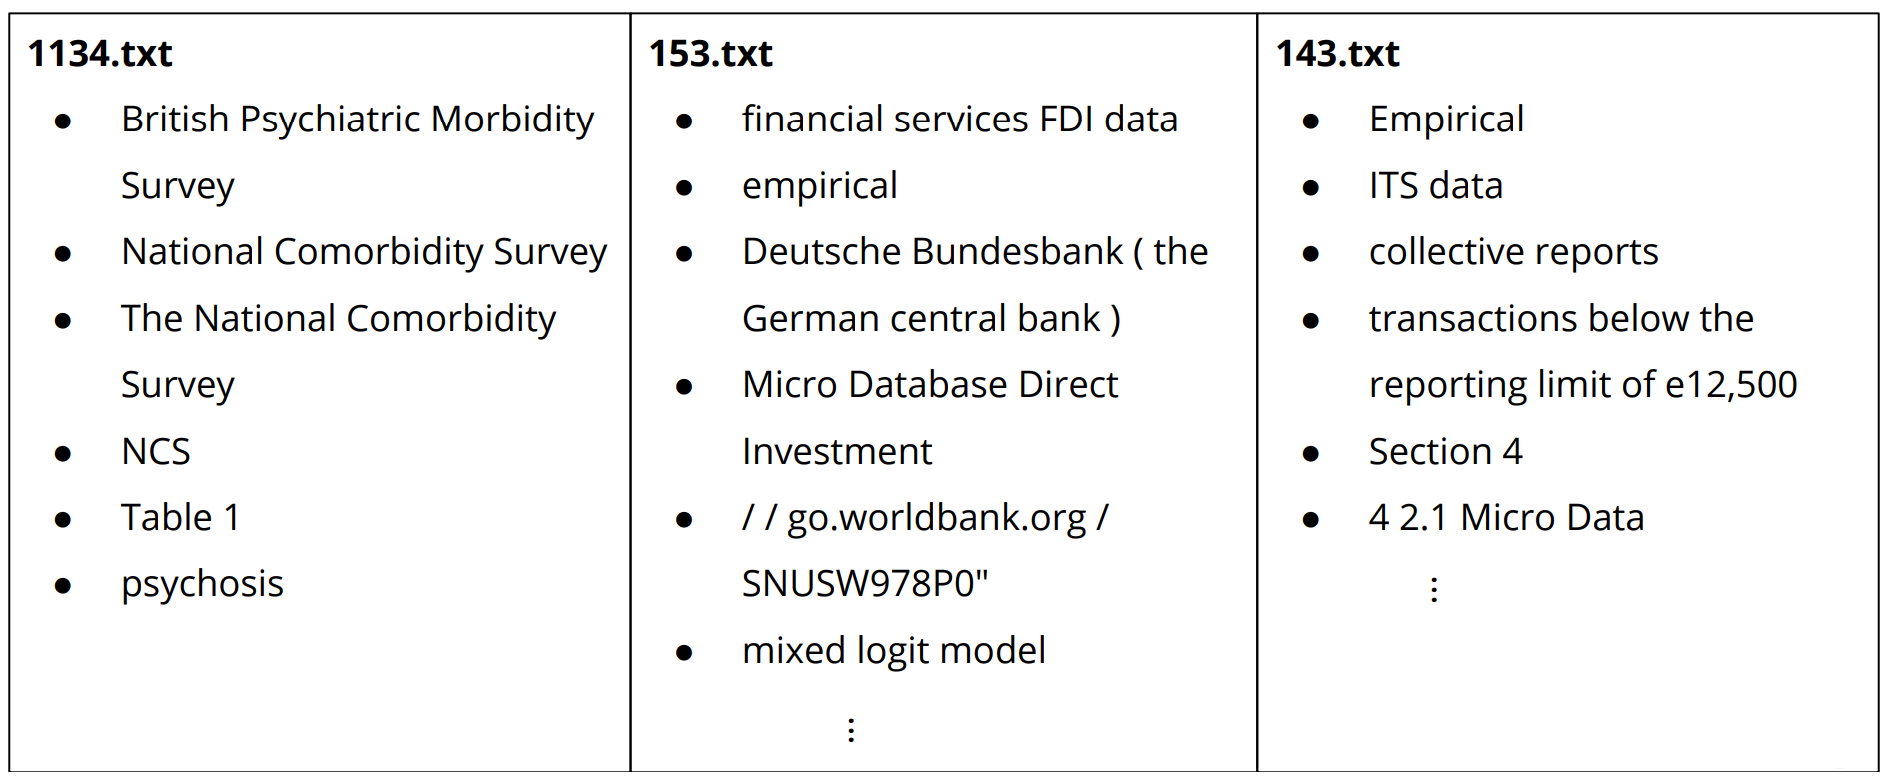
\includegraphics[width = 8cm]{phase1+querygen.png}
    \caption{Results from Document QA + query generation module}
    \label{fig:docqaquery}
\end{figure}

We believed that the reason of these noises is the several query terms potentially retrieve wrong answers. For example, we have a query term \textit{"study"} to retrieve dataset mentions such as \textit{"ANES 1952 Time Series Study"}. However, this term can also retrieve noises such as \textit{"empirical study"}. These kinds of query terms are still needed to retrieve various forms and types of dataset mentions, but clearly generate some noises.

\subsubsection{Document QA + query generation module + entity typing module}
Figure \ref{fig:docqaqueryentity} shows the results from 3 publications of phase 1 dev set with Document QA, query generation module, and entity typing module. Thanks to the entity typing module, we can see that most of noises from query generation module have disappeared. Although a few right answers such as \textit{"FDI data"} was filtered out and a few wrong answers such as \textit{"4.2.1 Micro Data"} was not, overall precision is adequately improved by entity typing module. In addition, our model in this setting could retrieve 526 answers (predictions) from 100 publications of phase 1 dev set.

\begin{figure}[!htb]
    \centering
    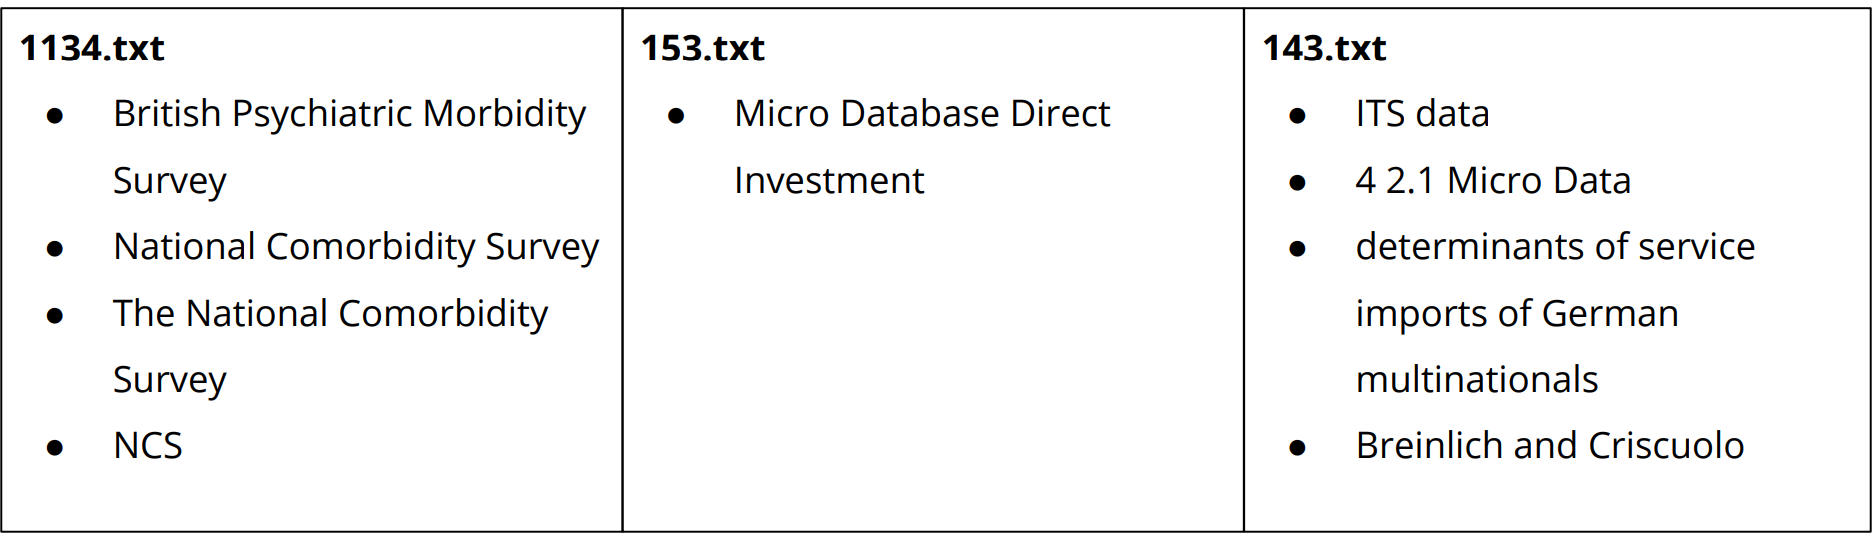
\includegraphics[width = 8cm]{phase1+querygen+entitytyping.png}
    \caption{Results from Document QA + query generation module + entity typing module}
    \label{fig:docqaqueryentity}
\end{figure}

\subsection{Research Fields Retrieval}
We randomly selected  20 publications from the training set of phase 1, since our model does not require any training. The model was able to correctly predict 11. The strongest point is that the model is able to predict research fields which are  significantly specific such as \textit{Home health nursing management}. Among the weak points of the model, it has problems when two research fields are similar or share subtopics. Moreover, sometimes it fails due to the fact that it tries to retrieve excessively specific fields while more general ones would be suitable.
%
%and For example, publication id 2238 is about \textit{Medicine: Body mass index, exercise and inflammatory markers} but the model returned \textit{Cardiovascular Technology}. Actually, it is close because the publication talks about cardiovascular issues, but not about \textit{Cardiovascular Technology}. If instead of trying to obtain a very specific field, we would have tried to obtain a more general one, we may have success. For example, in this case \textit{Medicine} would have been a right answer. We have several cases like this in our analysis and in addition to this, we also found a publication about immigration written in Portuguese. Our model only works in English so it got it wrong. Nevertheless, it tried its best and stated that the publication was about \textit{Spanish and Portuguese Studies}.

%We think that we can get better results if we also aim to return more general fields, so we expect to improve our accuracy till 0.7 approximately.

\subsection{Research Methods Retrieval}
20 random publications were selected from the training set of phase 2 and labelled. Our result is not as expected. The model is able to find proper research methods for 12 publications out of 20. For example, the model detects one of the research methods appeared in publication with id 15359 which is \textit{Factor analysis}. However, the results contain a notably amount of noise. For example, the document with id 10751, the model retrieves several wrong answers like: \textit{Reviews describe}, \textit{Composite materials}, \textit{Detailed databases}, etc. After analyzing this result, we found that the dataset we use for training is not appropriate for this task. For example, \textit{Reliability} and \textit{Independent variables} are marked as research methods, but actually they are not.

\section{Conclusions}
In this work we proposed three information retrieval models to mine information from scientific publications. One to retrieve the mentions of the datasets used, another one to retrieve the research field and the last one to retrieve the research methods. Our contributions are as follow. We modeled the dataset retrieval task as an QA problem. In order to solve this task, we proposed a query generation module and a filter using entity types. We also proposed to use Wikipedia articles to retrieve research fields from scientific publications. Finally, we proposed to model the research method retrieval task as an NER problem.


\section{Future Work}
This work is the very first step of the  
Coleridge Initiative to build an “Amazon.com” for data users and data producers. The next step is to construct a system that recommends datasets to researchers. We have a hypothesis that datasets depend on research fields and vice versa. For example, in the research field \textit{Question Answering}, a subfield of \textit{Natural Language Processing} and \textit{Computer Science}, the most commonly used dataset is SQuAD \cite{rajpurkar2016squad}. Therefore, according to our hypothesis, two publications using SQuAD are presumably to be in the same field,  \textit{Question Answering}. Based on this hypothesis, we intend to build hierarchical clusters of publications with the same research field. This way, a cluster will have publications with the same research field and similar datasets. As an example, the QA cluster will have papers about QA and those papers will use similar datasets like SQuAD and TriviaQA \cite{joshi2017triviaqa}. With these clusters, the system will be able to recommend datasets to data users. For example, if a publication is in the \textit{Question Answering} field, the proposed system would be able to recommend the authors SQuAD and TriviaQA. Moreover, it would be able to recommend to data producers fields with a lack of datasets.

In addition, we also need to improve the performance of the models we built. For example, since we used a pretrained model in Document QA we think we could not exploit the whole potential of this system, so we would like to train our own model using a training set of publications.  

% include your own bib file like this:
%\bibliographystyle{acl}
%\bibliography{acl2015}

\bibliographystyle{acl}
\bibliography{bibliography}


\end{document}
